% \begin{figure}[t]
%     \centering
%     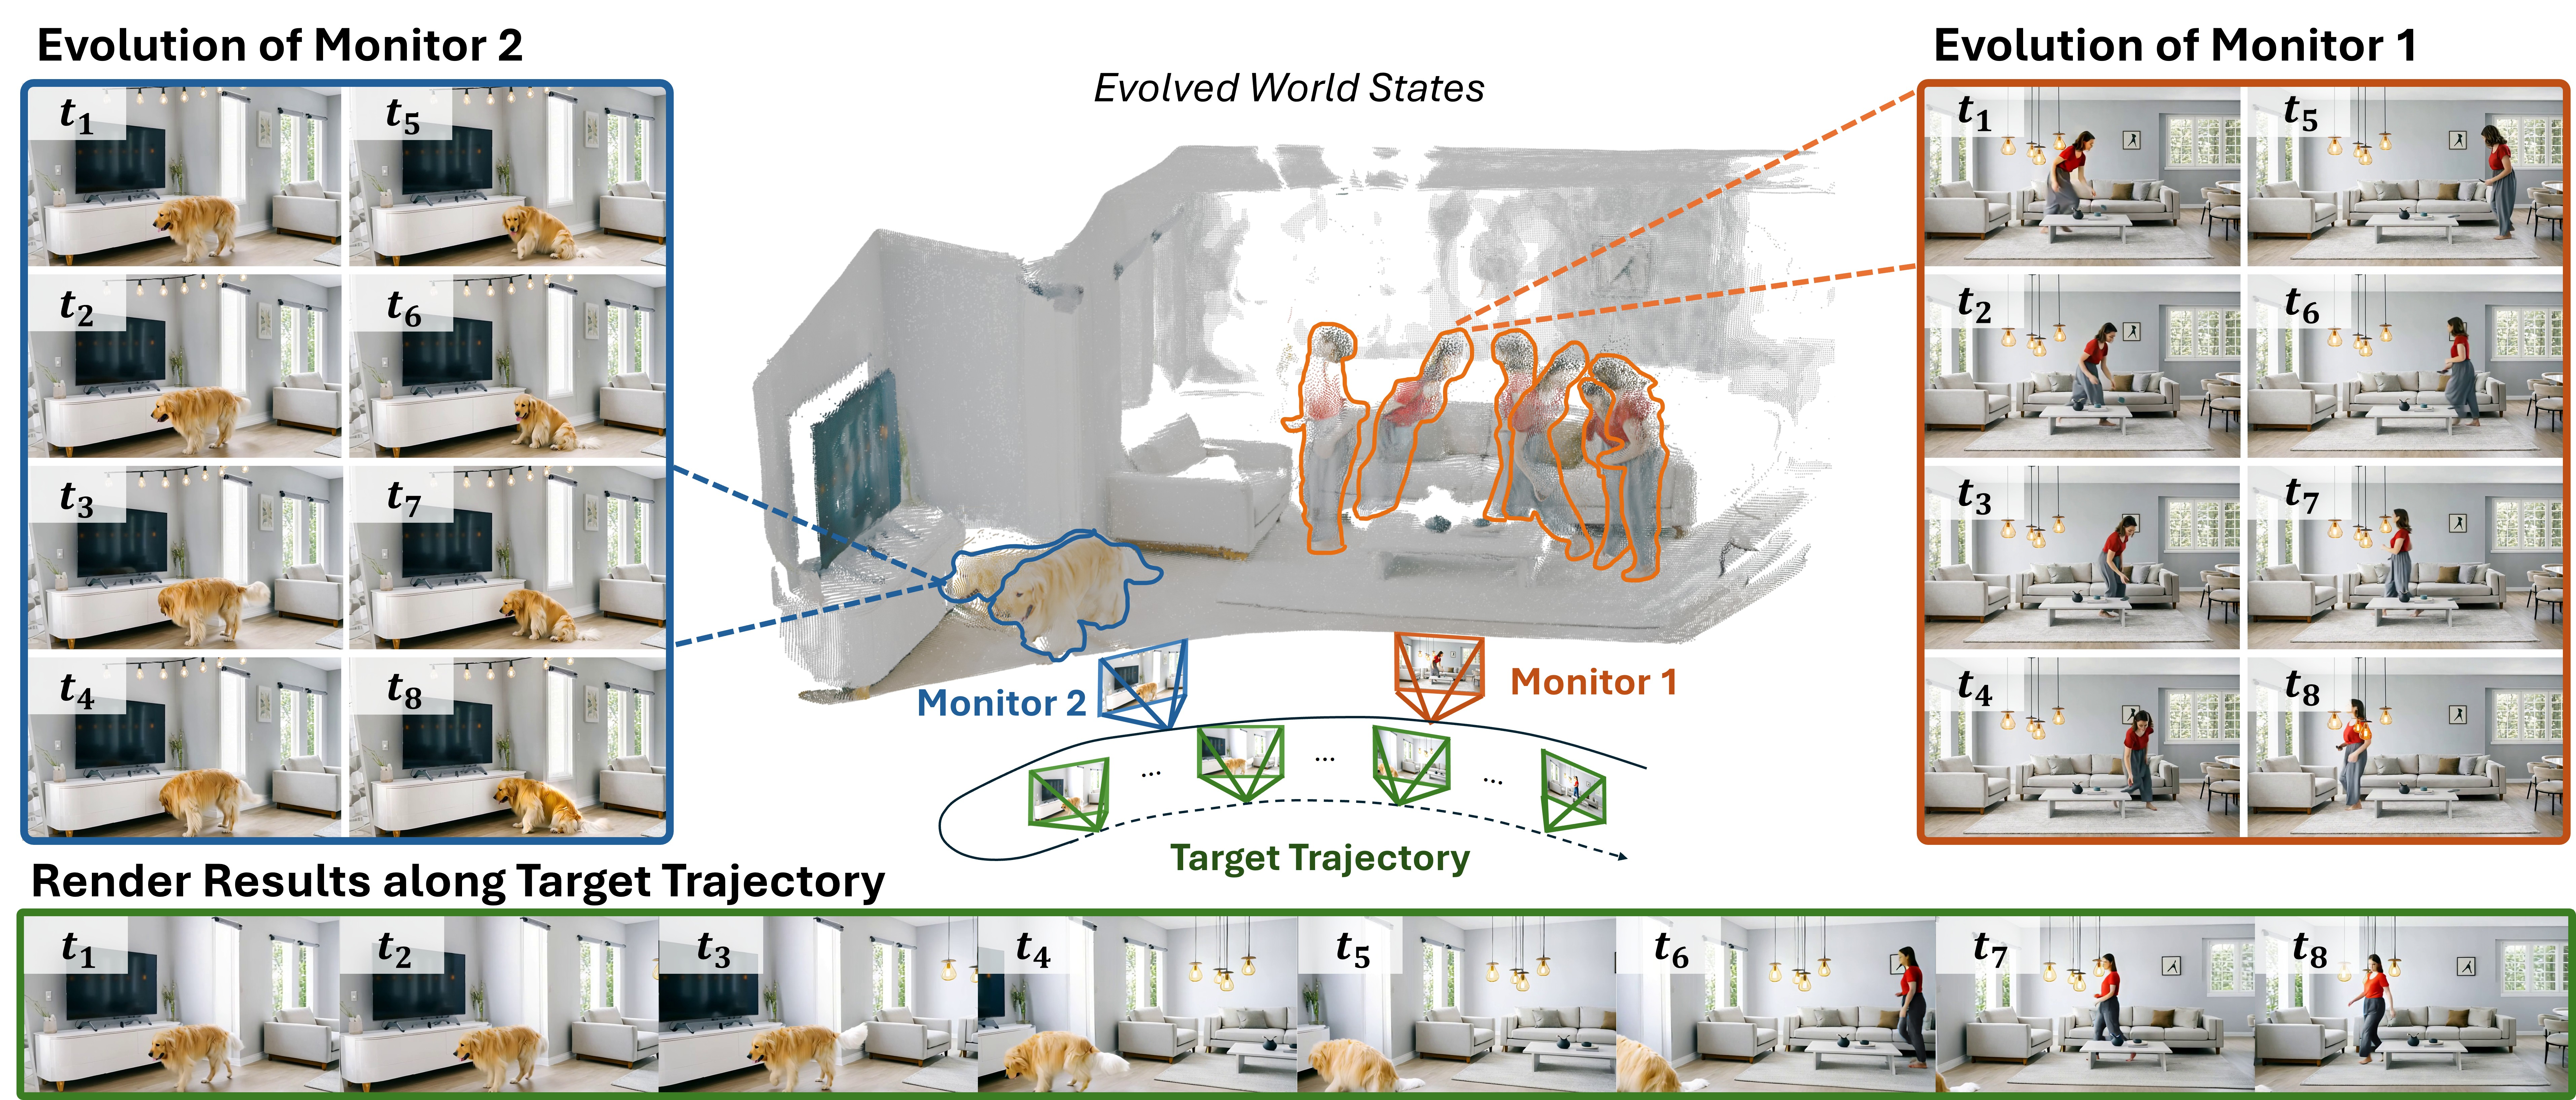
\includegraphics[width=1\linewidth]{imgs/teaser.jpg}
%     \caption{\textbf{LiveWorld enables persistent out-of-sight dynamics.} Instead of freezing unobserved regions, our framework explicitly decouples world evolution from observation rendering. We register stationary \textit{Monitors} to autonomously fast-forward the temporal progression of active entities (e.g., the dog and the person) in the background. As the observer explores the scene along the target trajectory (green cameras), our state-aware renderer projects the continuously evolved world states to synthesize the final observation. This ensures that dynamic events progress naturally, accurately reflecting the elapsed time even when entities are completely out of the observer's view.}
%     \label{fig:placeholder}
% \end{figure}

% \maketitle

\begin{center}
    \vspace{-5mm}
    \centering
    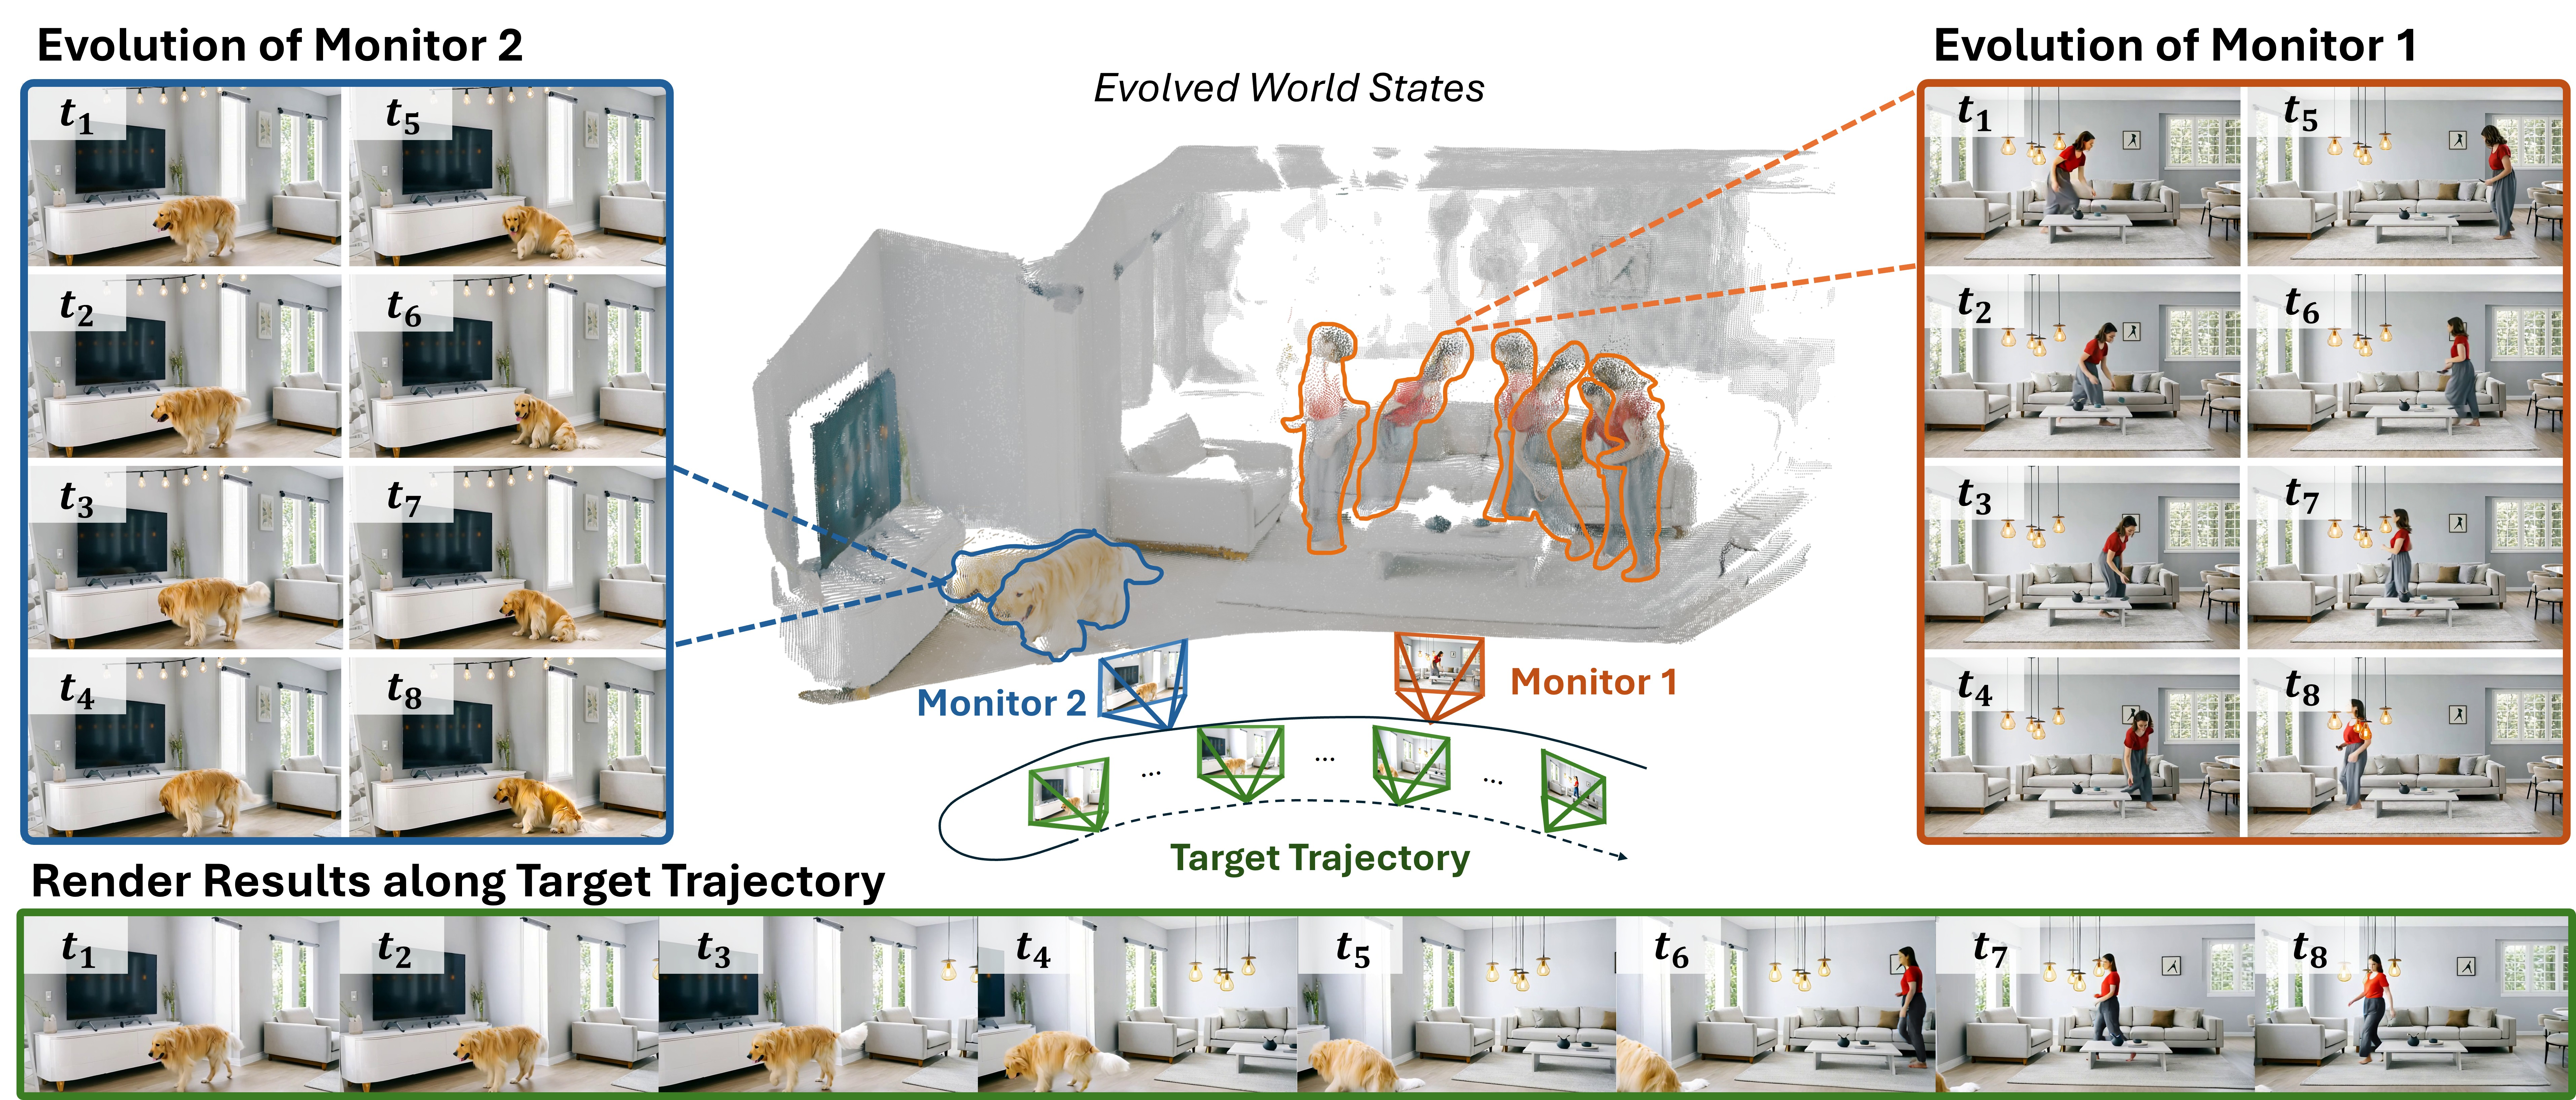
\includegraphics[width=\linewidth]{imgs/teaser.jpg}
    \vspace{-5mm}
    \captionof{figure}{\textbf{LiveWorld enables persistent out-of-sight dynamics.} Instead of freezing unobserved regions, our framework explicitly decouples world evolution from observation rendering. We register stationary \textit{Monitors} to autonomously fast-forward the temporal progression of active entities (e.g., the dog and the person) in the background. As the observer explores the scene along the target trajectory (green cameras), our state-aware renderer projects the continuously evolved world states to synthesize the final observation. This ensures that dynamic events progress naturally, accurately reflecting the elapsed time even when entities are completely out of the observer's view.}
    \label{fig:teaser}
    % \vspace{-2mm}
\end{center}

\begin{abstract}
\vspace{-2mm}

Recent generative video world models aim to simulate visual environment evolution, allowing an observer to interactively explore the scene via camera control. However, they implicitly assume that the world only evolves within the observer's field of view. Once an object leaves the observer’s view, its state is ``frozen'' in memory, and revisiting the same region later often fails to reflect events that should have occurred in the meantime. In this work, we identify and formalize this overlooked limitation as the ``out-of-sight dynamics'' problem, which impedes video world models from representing a continuously evolving world. To address this issue, we propose LiveWorld, a novel framework that extends video world models to support persistent world evolution. Instead of treating the world as static observational memory, LiveWorld models a persistent global state composed of a static 3D background and dynamic entities that continue evolving even when unobserved. To maintain these unseen dynamics, LiveWorld introduces a monitor-based mechanism that autonomously simulates the temporal progression of active entities and synchronizes their evolved states upon revisiting, ensuring spatially coherent rendering. For evaluation, we further introduce LiveBench, a dedicated benchmark for the task of maintaining out-of-sight dynamics. Extensive experiments show that LiveWorld enables persistent event evolution and long-term scene consistency, bridging the gap between existing 2D observation-based memory and true 4D dynamic world simulation. 
The baseline and benchmark will be publicly available.

\vspace{-0.5mm}
\end{abstract}
